The Horse Racing Tournament Management System (HRTMS) is a comprehensive web-based application designed to digitize and optimize the operational workflows of horse racing tournament organizations, race scheduling, and spectator participation.

\begin{itemize}
    \item \textbf{Operational Environment}:
    \begin{itemize}
        \item \textbf{Platform}: Web-based application accessible via standard web browsers (Chrome, Edge, Firefox, Safari).
        \item \textbf{Connectivity}: Requires a stable Internet connection to function (no offline mode).
        \item \textbf{Infrastructure}: Powered by a FastAPI backend API and a Next.js frontend, utilizing Microsoft SQL Server for the database.
    \end{itemize}
    
    \item \textbf{Anticipated Users}:
    \begin{itemize}
        \item \textbf{Internal Users}: Administrator and Race Referees.
        \item \textbf{External Users}: Horse Owners, Jockeys, and Spectators.
    \end{itemize}
    
    \item \textbf{Constraints \& Assumptions}:
    \begin{itemize}
        \item \textbf{Language}: The system database and interface support UTF-8 encoding for Vietnamese characters, with localized date/time formatting.
        \item \textbf{Compliance}: Complies with user account data privacy and local tournament scheduling rules in Vietnam.
        \item \textbf{Scope Limitation}: Does not support actual financial betting transactions; spectator predictions use virtual reward points only. Timezone handling is restricted to \texttt{Asia/Ho\_Chi\_Minh}.
    \end{itemize}
    
    \item \textbf{Dependencies}:
    \begin{itemize}
        \item Relies on local Python environment libraries (\texttt{pyodbc}, \texttt{SQLAlchemy}, \texttt{FastAPI}).
        \item Requires a configured Microsoft SQL Server database.
    \end{itemize}
\end{itemize}

\subsection{System Context Diagram}

The system context diagram below defines the boundaries and exchanges between the Horse Racing Tournament Management System and its external entities:

\begin{figure}[H]
    \centering
    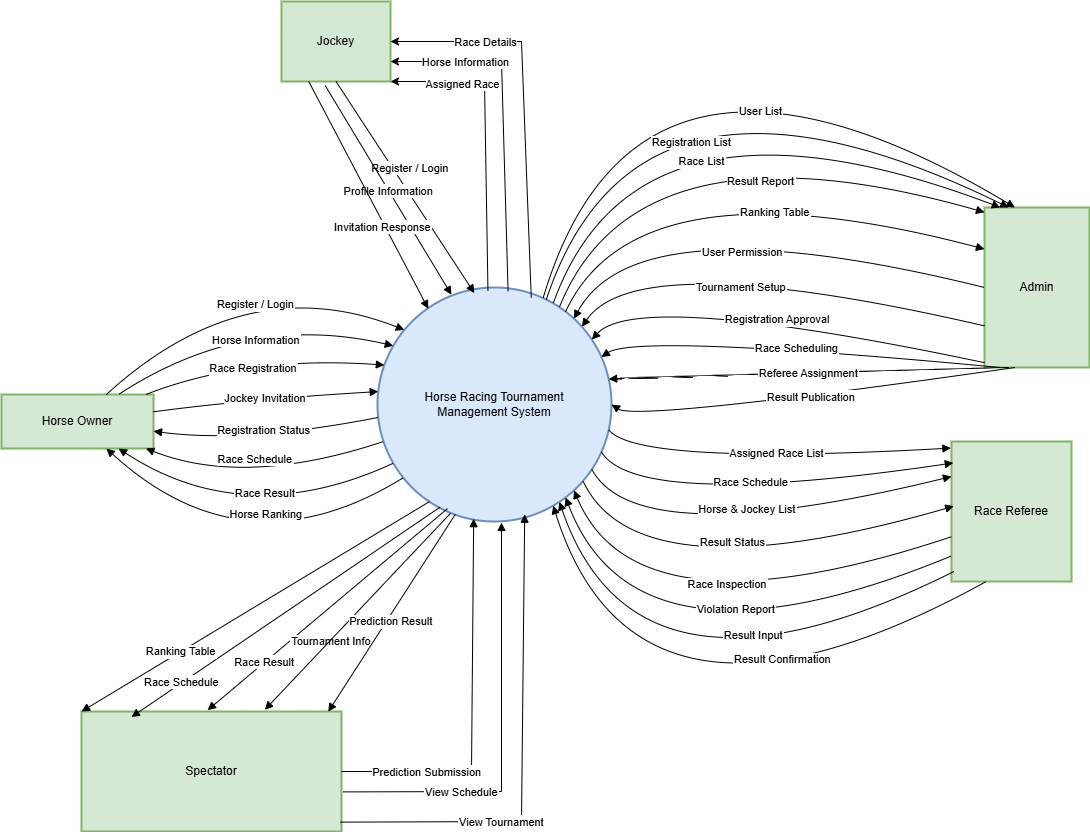
\includegraphics[width=0.95\textwidth]{figures/context_diagram.png}
    \caption{System Context Diagram}
    \label{fig:context_diagram}
\end{figure}

\subsection{Interaction Data Flows}

The data interactions between the system and each external actor are defined as follows:

\begin{itemize}
    \item \textbf{Horse Owner}:
    \begin{itemize}
        \item \textit{Data Input to System}: Register / Login, Horse Information, Race Registration, and Jockey Invitation.
        \item \textit{Data Output from System}: Registration Status, Race Schedule, Race Result, and Horse Ranking.
    \end{itemize}
    
    \item \textbf{Jockey}:
    \begin{itemize}
        \item \textit{Data Input to System}: Register / Login, Profile Information, and Invitation Response.
        \item \textit{Data Output from System}: Assigned Race, Race Details, and Horse Information.
    \end{itemize}
    
    \item \textbf{Administrator (Admin)}:
    \begin{itemize}
        \item \textit{Data Input to System}: User Permission, Tournament Setup, Registration Approval, Race Scheduling, Referee Assignment, and Result Publication.
        \item \textit{Data Output from System}: User List, Registration List, Race List, Result Report, and Ranking Table.
    \end{itemize}
    
    \item \textbf{Race Referee}:
    \begin{itemize}
        \item \textit{Data Input to System}: Race Inspection, Violation Report, Result Input, and Result Confirmation.
        \item \textit{Data Output from System}: Assigned Race List, Race Schedule, Horse \& Jockey List, and Result Status.
    \end{itemize}
    
    \item \textbf{Spectator}:
    \begin{itemize}
        \item \textit{Data Input to System}: View Tournament, Prediction Submission, and View Schedule.
        \item \textit{Data Output from System}: Tournament Info, Race Schedule, Race Result, Ranking Table, and Prediction Result.
    \end{itemize}
\end{itemize}
